% Options for packages loaded elsewhere
\PassOptionsToPackage{unicode}{hyperref}
\PassOptionsToPackage{hyphens}{url}
%
\documentclass[
]{article}
\usepackage{amsmath,amssymb}
\usepackage{iftex}
\ifPDFTeX
  \usepackage[T1]{fontenc}
  \usepackage[utf8]{inputenc}
  \usepackage{textcomp} % provide euro and other symbols
\else % if luatex or xetex
  \usepackage{unicode-math} % this also loads fontspec
  \defaultfontfeatures{Scale=MatchLowercase}
  \defaultfontfeatures[\rmfamily]{Ligatures=TeX,Scale=1}
\fi
\usepackage{lmodern}
\ifPDFTeX\else
  % xetex/luatex font selection
\fi
% Use upquote if available, for straight quotes in verbatim environments
\IfFileExists{upquote.sty}{\usepackage{upquote}}{}
\IfFileExists{microtype.sty}{% use microtype if available
  \usepackage[]{microtype}
  \UseMicrotypeSet[protrusion]{basicmath} % disable protrusion for tt fonts
}{}
\makeatletter
\@ifundefined{KOMAClassName}{% if non-KOMA class
  \IfFileExists{parskip.sty}{%
    \usepackage{parskip}
  }{% else
    \setlength{\parindent}{0pt}
    \setlength{\parskip}{6pt plus 2pt minus 1pt}}
}{% if KOMA class
  \KOMAoptions{parskip=half}}
\makeatother
\usepackage{xcolor}
\usepackage[margin=1in]{geometry}
\usepackage{color}
\usepackage{fancyvrb}
\newcommand{\VerbBar}{|}
\newcommand{\VERB}{\Verb[commandchars=\\\{\}]}
\DefineVerbatimEnvironment{Highlighting}{Verbatim}{commandchars=\\\{\}}
% Add ',fontsize=\small' for more characters per line
\usepackage{framed}
\definecolor{shadecolor}{RGB}{248,248,248}
\newenvironment{Shaded}{\begin{snugshade}}{\end{snugshade}}
\newcommand{\AlertTok}[1]{\textcolor[rgb]{0.94,0.16,0.16}{#1}}
\newcommand{\AnnotationTok}[1]{\textcolor[rgb]{0.56,0.35,0.01}{\textbf{\textit{#1}}}}
\newcommand{\AttributeTok}[1]{\textcolor[rgb]{0.13,0.29,0.53}{#1}}
\newcommand{\BaseNTok}[1]{\textcolor[rgb]{0.00,0.00,0.81}{#1}}
\newcommand{\BuiltInTok}[1]{#1}
\newcommand{\CharTok}[1]{\textcolor[rgb]{0.31,0.60,0.02}{#1}}
\newcommand{\CommentTok}[1]{\textcolor[rgb]{0.56,0.35,0.01}{\textit{#1}}}
\newcommand{\CommentVarTok}[1]{\textcolor[rgb]{0.56,0.35,0.01}{\textbf{\textit{#1}}}}
\newcommand{\ConstantTok}[1]{\textcolor[rgb]{0.56,0.35,0.01}{#1}}
\newcommand{\ControlFlowTok}[1]{\textcolor[rgb]{0.13,0.29,0.53}{\textbf{#1}}}
\newcommand{\DataTypeTok}[1]{\textcolor[rgb]{0.13,0.29,0.53}{#1}}
\newcommand{\DecValTok}[1]{\textcolor[rgb]{0.00,0.00,0.81}{#1}}
\newcommand{\DocumentationTok}[1]{\textcolor[rgb]{0.56,0.35,0.01}{\textbf{\textit{#1}}}}
\newcommand{\ErrorTok}[1]{\textcolor[rgb]{0.64,0.00,0.00}{\textbf{#1}}}
\newcommand{\ExtensionTok}[1]{#1}
\newcommand{\FloatTok}[1]{\textcolor[rgb]{0.00,0.00,0.81}{#1}}
\newcommand{\FunctionTok}[1]{\textcolor[rgb]{0.13,0.29,0.53}{\textbf{#1}}}
\newcommand{\ImportTok}[1]{#1}
\newcommand{\InformationTok}[1]{\textcolor[rgb]{0.56,0.35,0.01}{\textbf{\textit{#1}}}}
\newcommand{\KeywordTok}[1]{\textcolor[rgb]{0.13,0.29,0.53}{\textbf{#1}}}
\newcommand{\NormalTok}[1]{#1}
\newcommand{\OperatorTok}[1]{\textcolor[rgb]{0.81,0.36,0.00}{\textbf{#1}}}
\newcommand{\OtherTok}[1]{\textcolor[rgb]{0.56,0.35,0.01}{#1}}
\newcommand{\PreprocessorTok}[1]{\textcolor[rgb]{0.56,0.35,0.01}{\textit{#1}}}
\newcommand{\RegionMarkerTok}[1]{#1}
\newcommand{\SpecialCharTok}[1]{\textcolor[rgb]{0.81,0.36,0.00}{\textbf{#1}}}
\newcommand{\SpecialStringTok}[1]{\textcolor[rgb]{0.31,0.60,0.02}{#1}}
\newcommand{\StringTok}[1]{\textcolor[rgb]{0.31,0.60,0.02}{#1}}
\newcommand{\VariableTok}[1]{\textcolor[rgb]{0.00,0.00,0.00}{#1}}
\newcommand{\VerbatimStringTok}[1]{\textcolor[rgb]{0.31,0.60,0.02}{#1}}
\newcommand{\WarningTok}[1]{\textcolor[rgb]{0.56,0.35,0.01}{\textbf{\textit{#1}}}}
\usepackage{graphicx}
\makeatletter
\def\maxwidth{\ifdim\Gin@nat@width>\linewidth\linewidth\else\Gin@nat@width\fi}
\def\maxheight{\ifdim\Gin@nat@height>\textheight\textheight\else\Gin@nat@height\fi}
\makeatother
% Scale images if necessary, so that they will not overflow the page
% margins by default, and it is still possible to overwrite the defaults
% using explicit options in \includegraphics[width, height, ...]{}
\setkeys{Gin}{width=\maxwidth,height=\maxheight,keepaspectratio}
% Set default figure placement to htbp
\makeatletter
\def\fps@figure{htbp}
\makeatother
\setlength{\emergencystretch}{3em} % prevent overfull lines
\providecommand{\tightlist}{%
  \setlength{\itemsep}{0pt}\setlength{\parskip}{0pt}}
\setcounter{secnumdepth}{-\maxdimen} % remove section numbering
\ifLuaTeX
  \usepackage{selnolig}  % disable illegal ligatures
\fi
\usepackage{bookmark}
\IfFileExists{xurl.sty}{\usepackage{xurl}}{} % add URL line breaks if available
\urlstyle{same}
\hypersetup{
  pdftitle={ANÁLISIS DE LA CORRELACIÓN ENTRE LA INFLACIÓN Y LA PERCEPCIÓN DE CORRUPCIÓN},
  pdfauthor={Rubén Valverde Romero},
  hidelinks,
  pdfcreator={LaTeX via pandoc}}

\title{ANÁLISIS DE LA CORRELACIÓN ENTRE LA INFLACIÓN Y LA PERCEPCIÓN DE
CORRUPCIÓN}
\author{Rubén Valverde Romero}
\date{2024-10-19}

\begin{document}
\maketitle

{
\setcounter{tocdepth}{2}
\tableofcontents
}
\subsection{Introducción}\label{introduccion}

El objetivo de este informe es analizar la relación entre la inflación y
la corrupción.

\subsection{Limpieza de datos}\label{limpieza-de-datos}

\subsubsection{Carga y Visualización del
DataFrame}\label{carga-y-visualizacion-del-dataframe}

\begin{Shaded}
\begin{Highlighting}[]
\NormalTok{df }\OtherTok{\textless{}{-}} \FunctionTok{read.csv}\NormalTok{(}\StringTok{"inflation\_corruption\_1995\_2023\_Ruben\_Valverde.csv"}\NormalTok{)}
\FunctionTok{head}\NormalTok{(df[}\DecValTok{0}\SpecialCharTok{:}\DecValTok{6}\NormalTok{])}
\end{Highlighting}
\end{Shaded}

\begin{verbatim}
##       country iso region inflation_2023 score_2023 rank_2023
## 1 Afghanistan AFG     AP        no data         20       162
## 2     Albania ALB    ECA            4.8         37        98
## 3     Algeria DZA   MENA            9.3         36       104
## 4      Angola AGO    SSA           13.6         33       121
## 5   Argentina ARG    AME          133.5         37        98
## 6     Armenia ARM    ECA              2         47        62
\end{verbatim}

\begin{Shaded}
\begin{Highlighting}[]
\CommentTok{\# Nota: El resto de columnas son repeticiones de las columnas 3, 4 y 5 por lo que mostrarlas no aportan más información y empeoran la estética}
\end{Highlighting}
\end{Shaded}

\subsubsection{Reemplazo de Valores ``no data'' por
NA}\label{reemplazo-de-valores-no-data-por-na}

\begin{Shaded}
\begin{Highlighting}[]
\CommentTok{\# Contar valores "no data" en cada columna}
\NormalTok{inflation }\OtherTok{\textless{}{-}}\NormalTok{ df[, }\FunctionTok{grepl}\NormalTok{(}\StringTok{"inflation"}\NormalTok{, }\FunctionTok{names}\NormalTok{(df))]}
\NormalTok{no\_data\_count }\OtherTok{\textless{}{-}} \FunctionTok{colSums}\NormalTok{(inflation }\SpecialCharTok{==} \StringTok{"no data"}\NormalTok{, }\AttributeTok{na.rm =} \ConstantTok{TRUE}\NormalTok{)}
\FunctionTok{print}\NormalTok{(}\FunctionTok{paste}\NormalTok{(}\StringTok{"Hay un total de"}\NormalTok{, }\FunctionTok{sum}\NormalTok{(no\_data\_count), }\StringTok{"valores \textquotesingle{}no data\textquotesingle{}"}\NormalTok{))}
\end{Highlighting}
\end{Shaded}

\begin{verbatim}
## [1] "Hay un total de 128 valores 'no data'"
\end{verbatim}

\begin{Shaded}
\begin{Highlighting}[]
\CommentTok{\# Reemplazar los valores "no data" por NA en todo el DataFrame porque da problemas al conteo}
\NormalTok{df[df }\SpecialCharTok{==} \StringTok{"no data"}\NormalTok{] }\OtherTok{\textless{}{-}} \ConstantTok{NA}
\end{Highlighting}
\end{Shaded}

\subsubsection{Conversión de Columnas a
Numérico}\label{conversion-de-columnas-a-numerico}

\begin{Shaded}
\begin{Highlighting}[]
\CommentTok{\# Convertir las columnas de inflación de 1995 a 2023 a valores numéricos}
\ControlFlowTok{for}\NormalTok{ (year }\ControlFlowTok{in} \DecValTok{1995}\SpecialCharTok{:}\DecValTok{2023}\NormalTok{) \{}
\NormalTok{  column }\OtherTok{\textless{}{-}} \FunctionTok{paste}\NormalTok{(}\StringTok{"inflation"}\NormalTok{, year, }\AttributeTok{sep =} \StringTok{"\_"}\NormalTok{)}
\NormalTok{  df[[column]] }\OtherTok{\textless{}{-}} \FunctionTok{as.numeric}\NormalTok{(df[[column]])}
\NormalTok{\}}
\end{Highlighting}
\end{Shaded}

\subsubsection{Conteo de valores NA}\label{conteo-de-valores-na}

\begin{Shaded}
\begin{Highlighting}[]
\CommentTok{\# Contar y mostrar el número de valores nulos por columna}
\FunctionTok{print}\NormalTok{(}\FunctionTok{paste}\NormalTok{(}\StringTok{"Hay un total de"}\NormalTok{, }\FunctionTok{sum}\NormalTok{(}\FunctionTok{is.na}\NormalTok{(df)), }\StringTok{"valores nulos"}\NormalTok{))}
\end{Highlighting}
\end{Shaded}

\begin{verbatim}
## [1] "Hay un total de 2152 valores nulos"
\end{verbatim}

\subsection{Análisis de la Evolución de la Inflación Promedio Anual por
Región}\label{analisis-de-la-evoluciuxf3n-de-la-inflacion-promedio-anual-por-region}

\subsubsection{Formateo del DataFrame}\label{formateo-del-dataFrame}

\begin{Shaded}
\begin{Highlighting}[]
\CommentTok{\# Transformar el DataFrame de formato ancho a formato largo para poder analizar los datos de inflación, puntuación y rango a lo largo del tiempo posteriormente}
\NormalTok{df\_melted }\OtherTok{\textless{}{-}}\NormalTok{ df }\SpecialCharTok{\%\textgreater{}\%}
  \FunctionTok{pivot\_longer}\NormalTok{(}\AttributeTok{cols =} \FunctionTok{starts\_with}\NormalTok{(}\StringTok{"inflation\_"}\NormalTok{) }\SpecialCharTok{|} \FunctionTok{starts\_with}\NormalTok{(}\StringTok{"score\_"}\NormalTok{) }\SpecialCharTok{|} \FunctionTok{starts\_with}\NormalTok{(}\StringTok{"rank\_"}\NormalTok{),}
  \AttributeTok{names\_to =} \FunctionTok{c}\NormalTok{(}\StringTok{".value"}\NormalTok{, }\StringTok{"year"}\NormalTok{),}
  \AttributeTok{names\_sep =} \StringTok{"\_"}\NormalTok{) }\SpecialCharTok{\%\textgreater{}\%}
\FunctionTok{select}\NormalTok{(country, iso, region, year, inflation, score, rank)}

\CommentTok{\# Convertir las columnas \textquotesingle{}inflation\textquotesingle{}, \textquotesingle{}rank\textquotesingle{} y \textquotesingle{}score\textquotesingle{} a tipo numérico en el DataFrame df\_melted}
\NormalTok{df\_melted }\OtherTok{\textless{}{-}}\NormalTok{ df\_melted }\SpecialCharTok{\%\textgreater{}\%}
    \FunctionTok{mutate}\NormalTok{(}\FunctionTok{across}\NormalTok{(}\FunctionTok{c}\NormalTok{(inflation, rank, score), as.numeric))}
\FunctionTok{head}\NormalTok{(df\_melted)}
\end{Highlighting}
\end{Shaded}

\begin{verbatim}
## # A tibble: 6 x 7
##   country     iso   region year  inflation score  rank
##   <chr>       <chr> <chr>  <chr>     <dbl> <dbl> <dbl>
## 1 Afghanistan AFG   AP     2023       NA      20   162
## 2 Afghanistan AFG   AP     2022       10.6    24   150
## 3 Afghanistan AFG   AP     2021        7.8    16   174
## 4 Afghanistan AFG   AP     2020        5.6    19   165
## 5 Afghanistan AFG   AP     2019        2.3    16   173
## 6 Afghanistan AFG   AP     2018        0.6    16   172
\end{verbatim}

\begin{Shaded}
\begin{Highlighting}[]
\FunctionTok{summary}\NormalTok{(df\_melted)}
\end{Highlighting}
\end{Shaded}

\begin{verbatim}
##    country              iso               region              year          
##  Length:5133        Length:5133        Length:5133        Length:5133       
##  Class :character   Class :character   Class :character   Class :character  
##  Mode  :character   Mode  :character   Mode  :character   Mode  :character  
##                                                                             
##                                                                             
##                                                                             
##                                                                             
##    inflation            score            rank       
##  Min.   :  -72.70   Min.   : 0.40   Min.   :  1.00  
##  1st Qu.:    1.80   1st Qu.: 3.50   1st Qu.: 35.00  
##  Median :    4.00   Median :10.00   Median : 74.00  
##  Mean   :   28.78   Mean   :24.07   Mean   : 78.74  
##  3rd Qu.:    8.10   3rd Qu.:38.00   3rd Qu.:121.00  
##  Max.   :65374.10   Max.   :92.00   Max.   :182.00  
##  NA's   :128        NA's   :1012    NA's   :1012
\end{verbatim}

\subsubsection{Visualización de la
Inflación}\label{visualizacion-de-la-inflacion}

\begin{Shaded}
\begin{Highlighting}[]
\CommentTok{\# Crear un DataFrame con la inflación promedio anual por región}
\NormalTok{df\_avg\_inflation }\OtherTok{\textless{}{-}}\NormalTok{ df\_melted }\SpecialCharTok{\%\textgreater{}\%}
    \FunctionTok{group\_by}\NormalTok{(region, year) }\SpecialCharTok{\%\textgreater{}\%}
    \FunctionTok{summarise}\NormalTok{(}\AttributeTok{inflation =} \FunctionTok{median}\NormalTok{(inflation, }\AttributeTok{na.rm =} \ConstantTok{TRUE}\NormalTok{), }\AttributeTok{.groups =} \StringTok{"drop"}\NormalTok{) }\SpecialCharTok{\%\textgreater{}\%}
    \FunctionTok{ungroup}\NormalTok{()}

\CommentTok{\# Nota: Se utilizó la mediana en lugar del promedio para evitar que valores extremos afecten el resultado (Como la inflación de 1995 en Europa Oriental y Asia Central causada por Bulgaria y Venezuela en América)}

\CommentTok{\# Agregar un tema a los gráficos}
\FunctionTok{theme\_set}\NormalTok{(}\FunctionTok{theme\_bw}\NormalTok{())}

\CommentTok{\# Ajustar el tamaño de los gráficos}
\FunctionTok{options}\NormalTok{(}\AttributeTok{repr.plot.width=}\DecValTok{17}\NormalTok{, }\AttributeTok{repr.plot.height=}\DecValTok{7}\NormalTok{)}

\CommentTok{\# Hacer las letras más grandes y los títulos centrados}
\FunctionTok{theme\_update}\NormalTok{(}
    \AttributeTok{plot.title =} \FunctionTok{element\_text}\NormalTok{(}\AttributeTok{size =} \DecValTok{20}\NormalTok{, }\AttributeTok{hjust =} \FloatTok{0.5}\NormalTok{),}
    \AttributeTok{axis.title =} \FunctionTok{element\_text}\NormalTok{(}\AttributeTok{size =} \DecValTok{16}\NormalTok{),}
    \AttributeTok{axis.text =} \FunctionTok{element\_text}\NormalTok{(}\AttributeTok{size =} \DecValTok{14}\NormalTok{),}
    \AttributeTok{legend.title =} \FunctionTok{element\_text}\NormalTok{(}\AttributeTok{size =} \DecValTok{16}\NormalTok{),}
    \AttributeTok{legend.text =} \FunctionTok{element\_text}\NormalTok{(}\AttributeTok{size =} \DecValTok{14}\NormalTok{)}
\NormalTok{)}
\CommentTok{\# Crear el lineplot}
\NormalTok{A }\OtherTok{\textless{}{-}} \FunctionTok{ggplot}\NormalTok{(df\_avg\_inflation, }\FunctionTok{aes}\NormalTok{(}\AttributeTok{x =}\NormalTok{ year, }\AttributeTok{y =}\NormalTok{ inflation, }\AttributeTok{color =}\NormalTok{ region, }\AttributeTok{group =}\NormalTok{ region)) }\SpecialCharTok{+}
    \FunctionTok{geom\_line}\NormalTok{(}\AttributeTok{size=}\FloatTok{1.5}\NormalTok{) }\SpecialCharTok{+}
    \FunctionTok{scale\_y\_continuous}\NormalTok{(}\AttributeTok{limits =} \FunctionTok{c}\NormalTok{(}\DecValTok{0}\NormalTok{, }\DecValTok{23}\NormalTok{)) }\SpecialCharTok{+}
    \FunctionTok{geom\_text}\NormalTok{(}\AttributeTok{data =}\NormalTok{ df\_avg\_inflation }\SpecialCharTok{\%\textgreater{}\%} \FunctionTok{filter}\NormalTok{(inflation }\SpecialCharTok{\textgreater{}} \DecValTok{23}\NormalTok{),}
              \FunctionTok{aes}\NormalTok{(}\AttributeTok{label =} \FunctionTok{round}\NormalTok{(inflation, }\DecValTok{1}\NormalTok{), }\AttributeTok{y =} \DecValTok{23}\NormalTok{),}
              \AttributeTok{color =} \StringTok{"green"}\NormalTok{, }\AttributeTok{size =} \DecValTok{3}\NormalTok{, }\AttributeTok{vjust =} \SpecialCharTok{{-}}\FloatTok{0.5}\NormalTok{) }\SpecialCharTok{+}
    \FunctionTok{geom\_point}\NormalTok{(}\AttributeTok{size=}\DecValTok{3}\NormalTok{) }\SpecialCharTok{+}
    \FunctionTok{labs}\NormalTok{(}\AttributeTok{title =} \StringTok{"Evolución de la Inflación Promedio Anual por Región"}\NormalTok{,}
         \AttributeTok{x =} \StringTok{"Año"}\NormalTok{,}
         \AttributeTok{y =} \StringTok{"Inflación Promedio"}\NormalTok{,}
         \AttributeTok{color =} \StringTok{"Región"}\NormalTok{)}
\end{Highlighting}
\end{Shaded}

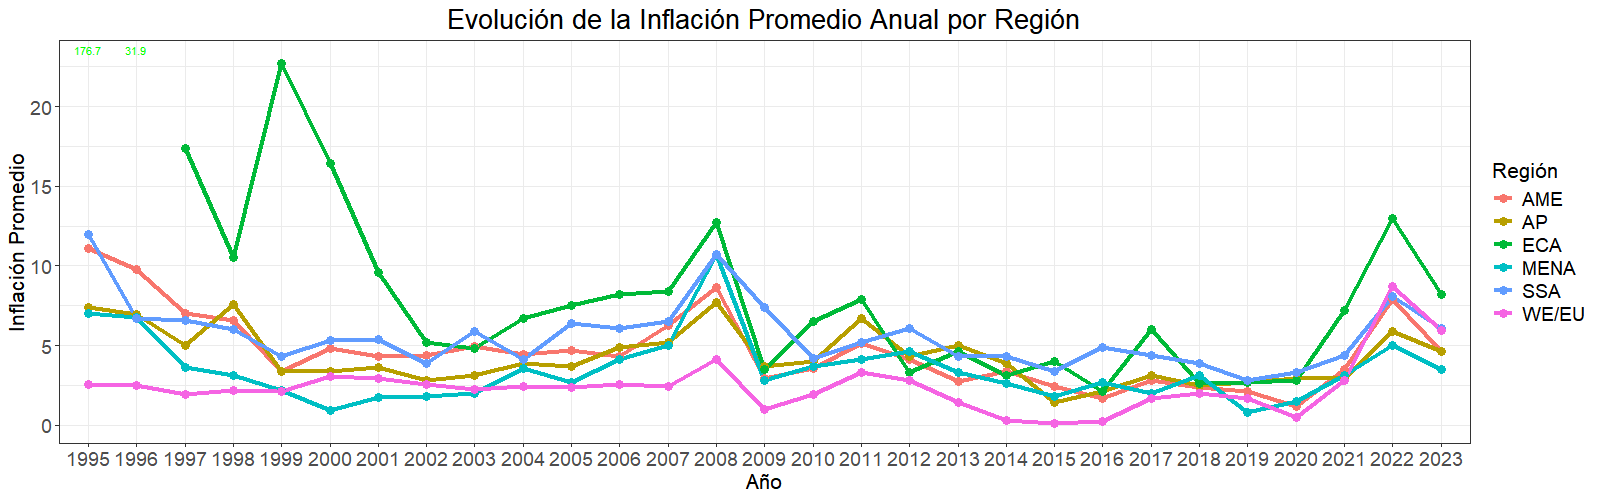
\includegraphics{Inflacion_Anual_Region.png}

\subsubsection{Análisis del Gráfico de Evolución de la Inflación
Promedio Anual por
Región}\label{analisis-del-grafico-de-evolucion-de-la-inflacion-promedio-anual-por-region}

El gráfico muestra la evolución de la inflación promedio anual por
región desde 1995 hasta 2023. A continuación, se presentan algunos
puntos clave observados en el gráfico:

\begin{enumerate}
\def\labelenumi{\arabic{enumi}.}
\tightlist
\item
  \textbf{América (AME)}:

  \begin{itemize}
  \tightlist
  \item
    Se observa una tendencia general a la baja en la inflación desde
    1995 hasta principios de la década de 2000.
  \item
    Sin embargo, hay picos significativos en ciertos años, lo que indica
    episodios de alta inflación en algunos países de la región.
  \item
    En los últimos años, la inflación ha vuelto a aumentar, alcanzando
    niveles preocupantes.
  \end{itemize}
\item
  \textbf{África Subsahariana (SSA)}:

  \begin{itemize}
  \tightlist
  \item
    La región muestra una tendencia similar a la de Latinoamérica, con
    una disminución de la inflación en la primera década del siglo XXI.
  \item
    A partir de 2010, la inflación ha mostrado una tendencia al alza,
    con picos notables en algunos años.
  \end{itemize}
\item
  \textbf{Asia-Pacífico (AP)}:

  \begin{itemize}
  \tightlist
  \item
    La región ha mantenido una inflación relativamente baja y estable en
    comparación con otras regiones.
  \item
    Aunque hay algunos picos, la inflación en Asia-Pacífico ha sido más
    controlada.
  \end{itemize}
\item
  \textbf{Europa Occidental y Union Europea (WE/EU)}:

  \begin{itemize}
  \tightlist
  \item
    Esta región ha experimentado una inflación muy baja y estable
    durante la mayor parte del período analizado.
  \item
    Sin embargo, en los últimos años se observa un aumento en la
    inflación, esto es debido al aumento maviso de la masa monetaria
    para superar la crisis del covid en un corto periodo de tiempo.
  \end{itemize}
\item
  \textbf{Medio Oriente y Norte de África (MENA)}:

  \begin{itemize}
  \tightlist
  \item
    La región muestra una inflación relativamente alta en comparación
    con Europa y Asia-Pacífico.
  \item
    Hay fluctuaciones significativas en la inflación, lo que indica
    inestabilidad económica en algunos países de la región.
  \end{itemize}
\item
  \textbf{Europa Oriental y Asia Central (ECA)}:

  \begin{itemize}
  \tightlist
  \item
    La región de ECA muestra una tendencia fluctuante en la inflación a
    lo largo de los años.
  \item
    Aunque algunos países han logrado mantener una inflación baja y
    estable, otros continúan enfrentando episodios de alta inflación.
  \end{itemize}
\end{enumerate}

\subsection{Análisis de la Evolución del Indice de Percepción de
Corrupción Promedio Anual (CPI) por
Región}\label{analisis-de-la-evolucion-del-indice-de-percepcion-de-corrupcion-promedio-anual-cpi-por-region}

\subsubsection{Adaptación al Cambio de Formato de
2012}\label{adaptacion-formato-cpi}

\begin{Shaded}
\begin{Highlighting}[]
\CommentTok{\# Al ejecutar el gráfico previamente se podia observar que el formato del CPI cambió en 2012, siendo 100 la puntuación máxima en lugar de 10.}
\NormalTok{df\_melted }\SpecialCharTok{\%\textgreater{}\%}
    \FunctionTok{filter}\NormalTok{(year }\SpecialCharTok{\%in\%} \FunctionTok{c}\NormalTok{(}\DecValTok{2010}\NormalTok{, }\DecValTok{2011}\NormalTok{, }\DecValTok{2012}\NormalTok{, }\DecValTok{2013}\NormalTok{)) }\SpecialCharTok{\%\textgreater{}\%}
    \FunctionTok{group\_by}\NormalTok{(region, year) }\SpecialCharTok{\%\textgreater{}\%}
    \FunctionTok{summarise}\NormalTok{(}\AttributeTok{score =} \FunctionTok{mean}\NormalTok{(score, }\AttributeTok{na.rm =} \ConstantTok{TRUE}\NormalTok{), }\AttributeTok{.groups =} \StringTok{"drop"}\NormalTok{) }\SpecialCharTok{\%\textgreater{}\%}
    \FunctionTok{head}\NormalTok{(}\DecValTok{4}\NormalTok{)}
\end{Highlighting}
\end{Shaded}

\begin{verbatim}
## # A tibble: 4 x 3
##   region year  score
##   <chr>  <chr> <dbl>
## 1 AME    2010   4.02
## 2 AME    2011   4.16
## 3 AME    2012  44.9 
## 4 AME    2013  44.3
\end{verbatim}

\begin{Shaded}
\begin{Highlighting}[]
\CommentTok{\# Multiplico por 10 el CPI de los años 1995 hasta 2011 para que estén en la misma escala que los años posteriores}
\NormalTok{df\_melted }\OtherTok{\textless{}{-}}\NormalTok{ df\_melted }\SpecialCharTok{\%\textgreater{}\%}
    \FunctionTok{mutate}\NormalTok{(}\AttributeTok{score =} \FunctionTok{ifelse}\NormalTok{(year }\SpecialCharTok{\textgreater{}=} \DecValTok{1995} \SpecialCharTok{\&}\NormalTok{ year }\SpecialCharTok{\textless{}=} \DecValTok{2011}\NormalTok{, score }\SpecialCharTok{*} \DecValTok{10}\NormalTok{, score))}
\end{Highlighting}
\end{Shaded}

\subsubsection{Calculo del CPI anual por
región}\label{calculo-del-cpi-anual-por-region}

\begin{Shaded}
\begin{Highlighting}[]
\CommentTok{\# Calcular el CPI promedio anual por región}
\NormalTok{df\_avg\_score }\OtherTok{\textless{}{-}}\NormalTok{ df\_melted }\SpecialCharTok{\%\textgreater{}\%}
    \FunctionTok{group\_by}\NormalTok{(region, year) }\SpecialCharTok{\%\textgreater{}\%}
    \FunctionTok{summarise}\NormalTok{(}\AttributeTok{score =} \FunctionTok{mean}\NormalTok{(score, }\AttributeTok{na.rm =} \ConstantTok{TRUE}\NormalTok{), }\AttributeTok{.groups =} \StringTok{"drop"}\NormalTok{) }\SpecialCharTok{\%\textgreater{}\%}
    \FunctionTok{ungroup}\NormalTok{()}

\CommentTok{\# Eliminar filas con valores nulos en la columna \textquotesingle{}score\textquotesingle{}, provocaban warnings}
\NormalTok{df\_avg\_score }\OtherTok{\textless{}{-}}\NormalTok{ df\_avg\_score }\SpecialCharTok{\%\textgreater{}\%} \FunctionTok{drop\_na}\NormalTok{(score)   }
\end{Highlighting}
\end{Shaded}

\subsubsection{Visualización del CPI}\label{visualizacion-del-cpi}

\begin{Shaded}
\begin{Highlighting}[]
\CommentTok{\# Crear el lineplot}
\NormalTok{A }\OtherTok{\textless{}{-}} \FunctionTok{ggplot}\NormalTok{(df\_avg\_score, }\FunctionTok{aes}\NormalTok{(}\AttributeTok{x =}\NormalTok{ year, }\AttributeTok{y =}\NormalTok{ score, }\AttributeTok{color =}\NormalTok{ region, }\AttributeTok{group =}\NormalTok{ region)) }\SpecialCharTok{+}
    \FunctionTok{geom\_line}\NormalTok{(}\AttributeTok{size=}\FloatTok{1.5}\NormalTok{) }\SpecialCharTok{+}
    \FunctionTok{geom\_point}\NormalTok{(}\AttributeTok{size=}\DecValTok{3}\NormalTok{) }\SpecialCharTok{+}
    \FunctionTok{labs}\NormalTok{(}\AttributeTok{title =} \StringTok{"Evolución del Indice de Percepción de Corrupción Promedio Anual (CPI) por Región"}\NormalTok{,}
         \AttributeTok{x =} \StringTok{"Año"}\NormalTok{,}
         \AttributeTok{y =} \StringTok{"CPI Promedio"}\NormalTok{,}
         \AttributeTok{color =} \StringTok{"Región"}\NormalTok{)}
\end{Highlighting}
\end{Shaded}

\includegraphics{CPI_Region_Año.png}

\subsubsection{Análisis del Gráfico de Evolución de la Puntuación de la
Percepción de Corrupción (CPI) Promedio Anual por
Región}\label{analisis-del-grafico-de-la-evolucion-del-indice-de-percepcion-de-corrupcion-promedio-anual-cpi-por-region}

El gráfico muestra la evolución de la puntuación de corrupción promedio
anual por región desde 1995 hasta 2023. A continuación, se presentan
algunos puntos clave observados en el gráfico:

\begin{enumerate}
\def\labelenumi{\arabic{enumi}.}
\tightlist
\item
  \textbf{América (AME)}:

  \begin{itemize}
  \tightlist
  \item
    La puntuación de corrupción en Latinoamérica ha mostrado una
    tendencia fluctuante a lo largo de los años.
  \item
    Aunque hay años en los que se observa una mejora en la puntuación,
    la región sigue enfrentando desafíos significativos en términos de
    corrupción.
  \end{itemize}
\item
  \textbf{África Subsahariana (SSA)}:

  \begin{itemize}
  \tightlist
  \item
    La región de África Subsahariana muestra una tendencia similar a la
    de Latinoamérica, con puntuaciones de corrupción que varían
    considerablemente a lo largo del tiempo.
  \item
    A pesar de algunos avances, la corrupción sigue siendo un problema
    persistente en muchos países de la región.
  \end{itemize}
\item
  \textbf{Asia-Pacífico (AP)}:

  \begin{itemize}
  \tightlist
  \item
    La región de Asia-Pacífico ha mantenido una puntuación de corrupción
    relativamente estable en comparación con otras regiones.
  \item
    Aunque hay algunos picos y valles, la puntuación de corrupción en
    Asia-Pacífico ha sido más controlada.
  \end{itemize}
\item
  \textbf{Europa Occidental y Union Europea (WE/EU)}:

  \begin{itemize}
  \tightlist
  \item
    Esta región ha experimentado una puntuación de corrupción
    relativamente baja y estable durante la mayor parte del período
    analizado.
  \item
    Sin embargo, en los últimos años se observa una ligera disminución
    en la puntuación, lo que podría indicar un aumento en los desafíos
    relacionados con la corrupción.
  \end{itemize}
\item
  \textbf{Medio Oriente y Norte de África (MENA)}:

  \begin{itemize}
  \tightlist
  \item
    La región de MENA muestra una puntuación de corrupción relativamente
    alta en comparación con Europa y Asia-Pacífico.
  \item
    Hay fluctuaciones significativas en la puntuación, lo que indica
    inestabilidad en la lucha contra la corrupción en algunos países de
    la región.
  \end{itemize}
\item
  \textbf{Europa Oriental y Asia Central (ECA)}:

  \begin{itemize}
  \tightlist
  \item
    La región de ECA muestra una tendencia fluctuante en la puntuación
    de corrupción a lo largo de los años.
  \item
    Aunque algunos países han logrado mejoras significativas, otros
    continúan enfrentando altos niveles de corrupción.
  \end{itemize}
\end{enumerate}

\subsection{Análisis de la Correlación entre la Puntuación de Corrupción
y la
Inflación}\label{analisis-de-la-correlacion-entre-la-puntuacion-de-corrupcion-y-la-inflacion}

\subsubsection{Calculo de valores medianos de inflación y medios de
puntuación de corrupción}\label{calculo-inflacion-cpi}

\begin{Shaded}
\begin{Highlighting}[]
\CommentTok{\# Calculo los valores medios de inflación y puntuación de corrupción por país}
\NormalTok{df\_avg }\OtherTok{\textless{}{-}}\NormalTok{ df\_melted }\SpecialCharTok{\%\textgreater{}\%}
    \FunctionTok{group\_by}\NormalTok{(country, region) }\SpecialCharTok{\%\textgreater{}\%} 
    \FunctionTok{summarise}\NormalTok{(}
        \AttributeTok{inflation =} \FunctionTok{median}\NormalTok{(inflation, }\AttributeTok{na.rm =} \ConstantTok{TRUE}\NormalTok{),}
        \AttributeTok{score =} \FunctionTok{mean}\NormalTok{(score, }\AttributeTok{na.rm =} \ConstantTok{TRUE}\NormalTok{), }\AttributeTok{.groups =} \StringTok{"drop"}
\NormalTok{    ) }\SpecialCharTok{\%\textgreater{}\%}
    \FunctionTok{arrange}\NormalTok{(region, country)}
    
\CommentTok{\# Nota1: ordeno por región y país para que el hue siga el mismo orden que el resto}
\CommentTok{\# Nota2: utilizo la mediana para la inflación para evitar que valores extremos como los de Bulgaria y Venezuela ya mencionados.}
\end{Highlighting}
\end{Shaded}

\subsubsection{Visualización de la
correlación}\label{visualizacion-correlacion}

\begin{Shaded}
\begin{Highlighting}[]
\CommentTok{\# Crear el scatter plot para visualizar la correlación entre inflación y puntuación de corrupción}
\CommentTok{\# Crear el scatter plot con una línea de regresión única para todas las regiones pero sin el scatter (Quiero una única linea de regresión)}
\NormalTok{A }\OtherTok{\textless{}{-}} \FunctionTok{ggplot}\NormalTok{(df\_avg, }\FunctionTok{aes}\NormalTok{(}\AttributeTok{x =}\NormalTok{ inflation, }\AttributeTok{y =}\NormalTok{ score, }\AttributeTok{color =}\NormalTok{ region)) }\SpecialCharTok{+}
    \FunctionTok{geom\_point}\NormalTok{(}\AttributeTok{size =} \DecValTok{3}\NormalTok{) }\SpecialCharTok{+}
    \FunctionTok{geom\_smooth}\NormalTok{(}\AttributeTok{method =} \StringTok{"lm"}\NormalTok{, }\AttributeTok{se =} \ConstantTok{FALSE}\NormalTok{, }\AttributeTok{linetype =} \StringTok{"dashed"}\NormalTok{, }\AttributeTok{size =} \FloatTok{2.5}\NormalTok{, }\AttributeTok{color =} \StringTok{"black"}\NormalTok{, }\AttributeTok{formula =}\NormalTok{ y }\SpecialCharTok{\textasciitilde{}}\NormalTok{ x) }\SpecialCharTok{+}
    \FunctionTok{labs}\NormalTok{(}
        \AttributeTok{title =} \StringTok{"Correlación entre Inflación y Puntuación de Corrupción por País"}\NormalTok{,}
        \AttributeTok{x =} \StringTok{"Inflación Mediana"}\NormalTok{,}
        \AttributeTok{y =} \StringTok{"Puntuación de Corrupción Promedio"}\NormalTok{,}
        \AttributeTok{color =} \StringTok{"Región"}
\NormalTok{    )}
\end{Highlighting}
\end{Shaded}

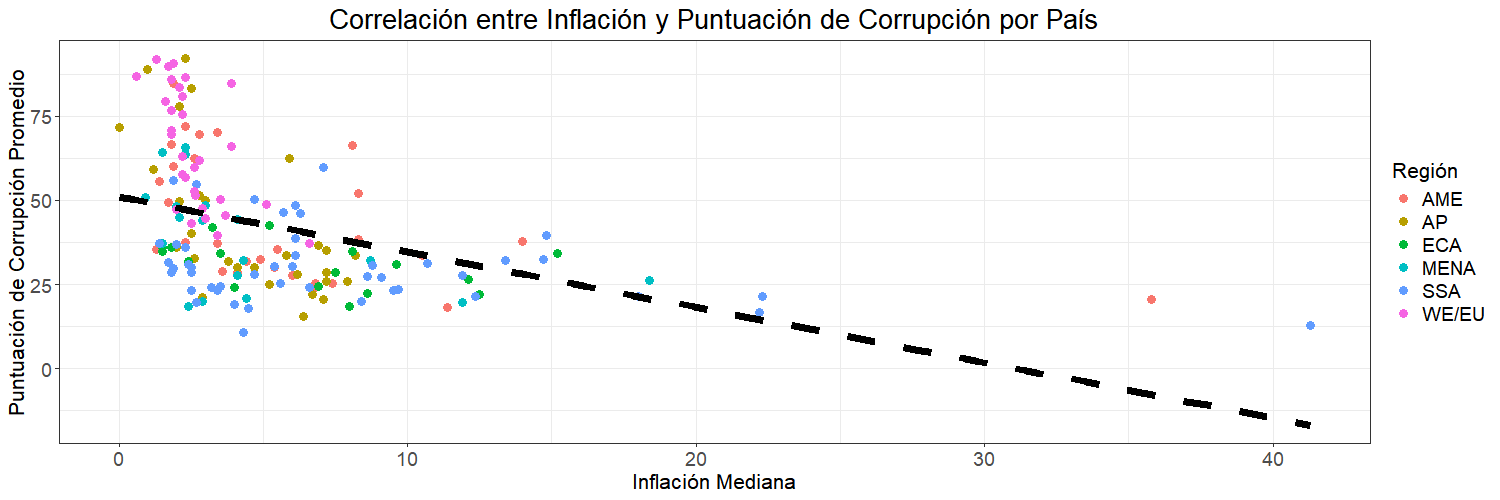
\includegraphics{Correlacion_CPI_Inflacion.png}

\subsubsection{Análisis del gráfico de la Correlación entre el CPI y la
Inflación}\label{analisis-del-grafico-correlacion-cpi-inflacion}

El scatterplot muestra la relación entre la inflación y la puntuación de
corrupción promedio por país. A continuación, se presentan algunos
puntos clave observados en el gráfico:

\begin{enumerate}
\def\labelenumi{\arabic{enumi}.}
\tightlist
\item
  \textbf{Tendencia General}:

  \begin{itemize}
  \tightlist
  \item
    Existe una tendencia negativa entre la inflación y la puntuación de
    corrupción. Esto sugiere que a medida que aumenta la inflación, la
    puntuación de corrupción tiende a disminuir, indicando mayores
    niveles de corrupción.
  \end{itemize}
\item
  \textbf{Regiones con Alta Inflación}:

  \begin{itemize}
  \tightlist
  \item
    Las regiones como Latinoamérica (AME) y África Subsahariana (SSA)
    muestran una mayor dispersión en los valores de inflación, con
    algunos países experimentando inflaciones extremadamente altas.
    Estos países también tienden a tener puntuaciones de corrupción más
    bajas, lo que indica altos niveles de corrupción.
  \end{itemize}
\item
  \textbf{Regiones con Baja Inflación}:

  \begin{itemize}
  \tightlist
  \item
    Europa Occidental, la Union Europea(WE/EU) y Asia-Pacífico (AP)
    muestran inflaciones relativamente bajas y puntuaciones de
    corrupción más altas, lo que indica menores niveles de corrupción.
    Esto sugiere una mejor gestión económica y políticas más efectivas
    contra la corrupción en estas regiones.
  \end{itemize}
\item
  \textbf{Línea de Tendencia}:

  \begin{itemize}
  \tightlist
  \item
    La línea de tendencia discontinua en el gráfico refuerza la relación
    negativa entre la inflación y la puntuación de corrupción. Aunque
    hay excepciones, la mayoría de los puntos siguen esta tendencia.
  \end{itemize}
\item
  \textbf{Valores Atípicos}:

  \begin{itemize}
  \tightlist
  \item
    Se eliminaron los valores atípicos de inflación (percentil 95) para
    obtener una representación más clara de la tendencia general. Los
    valores extremadamente altos de inflación empeoraban la
    visualización de la relación entre las variables.
  \end{itemize}
\end{enumerate}

En resumen, el gráfico sugiere que existe una correlación negativa entre
la inflación y la puntuación de corrupción. Las regiones con alta
inflación tienden a tener mayores niveles de corrupción, mientras que
las regiones con baja inflación muestran menores niveles de corrupción.
Este análisis destaca la importancia de la estabilidad económica y la
buena gobernanza en la retención del poder adquisitivo de la moneda.

\subsubsection{Coeficiente de Correlación de Spearman's
Rank}\label{spearman}

\begin{Shaded}
\begin{Highlighting}[]
\CommentTok{\# Calcular el coeficiente de correlación de Spearman}
\NormalTok{corr\_test }\OtherTok{\textless{}{-}} \FunctionTok{cor.test}\NormalTok{(df\_melted}\SpecialCharTok{$}\NormalTok{inflation, df\_melted}\SpecialCharTok{$}\NormalTok{score,}
                      \AttributeTok{method =} \StringTok{"spearman"}\NormalTok{, }\AttributeTok{use =} \StringTok{"complete.obs"}\NormalTok{,}
                      \AttributeTok{exact =} \ConstantTok{FALSE}\NormalTok{)}
\CommentTok{\# Nota: Utilizo el método de Spearman porque no se una distribución normal y hay valores extremos}
\CommentTok{\# Nota: Me saltaba el error de que no era posible calcular el coeficiente exacto, por lo que lo he puesto en FALSE, es decir, que no se calcula exactamente.}

\CommentTok{\# Definir el nivel de significancia}
\NormalTok{alpha }\OtherTok{\textless{}{-}} \FloatTok{0.05}

\CommentTok{\# Mostrar los resultados}
\FunctionTok{cat}\NormalTok{(}\StringTok{"Coeficiente de Correlación de Spearman\textquotesingle{}s Rank:"}\NormalTok{, corr\_test}\SpecialCharTok{$}\NormalTok{estimate, }\StringTok{"}\SpecialCharTok{\textbackslash{}n}\StringTok{"}\NormalTok{)}
\end{Highlighting}
\end{Shaded}

\begin{verbatim}
## Coeficiente de Correlación de Spearman's Rank: -0.4098749
\end{verbatim}

\begin{Shaded}
\begin{Highlighting}[]
\ControlFlowTok{if}\NormalTok{ (corr\_test}\SpecialCharTok{$}\NormalTok{p.value }\SpecialCharTok{\textless{}}\NormalTok{ alpha) \{}
  \FunctionTok{cat}\NormalTok{(}\StringTok{"p{-}valor:"}\NormalTok{, corr\_test}\SpecialCharTok{$}\NormalTok{p.value, }\StringTok{", Se rechaza la hipótesis nula}\SpecialCharTok{\textbackslash{}n}\StringTok{"}\NormalTok{)}
\NormalTok{\} }\ControlFlowTok{else}\NormalTok{ \{}
  \FunctionTok{cat}\NormalTok{(}\StringTok{"p{-}valor:"}\NormalTok{, corr\_test}\SpecialCharTok{$}\NormalTok{p.value, }\StringTok{", No se rechaza la hipótesis nula}\SpecialCharTok{\textbackslash{}n}\StringTok{"}\NormalTok{)}
\NormalTok{\}}
\end{Highlighting}
\end{Shaded}

\begin{verbatim}
## p-valor: 6.571181e-165 , Se rechaza la hipótesis nula
\end{verbatim}

\paragraph{Resultados:}\label{resultados}

El Coeficiente de Correlación de Spearman's Rank calculado entre las
columnas \texttt{inflation} y \texttt{score} ha arrojado los siguientes
resultados:

\begin{itemize}
\tightlist
\item
  \textbf{Coeficiente de Correlación de Spearman's Rank}: -0.4098749
\item
  \textbf{p-valor}: 6.571181e-165
\end{itemize}

\paragraph{Interpretación:}\label{interpretacion}

\begin{enumerate}
\def\labelenumi{\arabic{enumi}.}
\tightlist
\item
  \textbf{Coeficiente de Correlación}:

  \begin{itemize}
  \tightlist
  \item
    El valor del coeficiente de correlación de Spearman es -0.4098749,
    lo que indica una correlación negativa moderada entre la inflación y
    la puntuación de corrupción. Esto sugiere que, en general, a medida
    que aumenta la inflación, la puntuación de corrupción tiende a
    disminuir, lo que indica mayores niveles de corrupción.
  \end{itemize}
\item
  \textbf{p-valor}:

  \begin{itemize}
  \tightlist
  \item
    El \textbf{p-valor} obtenido es extremadamente bajo (6.571181e-165),
    lo que es mucho menor que el nivel de significancia comúnmente
    utilizado (\textbf{α} = 0.05). Esto significa que podemos rechazar
    la hipótesis nula de que no existe correlación entre la inflación y
    la puntuación de corrupción. En otras palabras, la correlación
    observada es estadísticamente significativa.
  \end{itemize}
\end{enumerate}

En resumen, los resultados del Coeficiente de Correlación de Spearman's
Rank sugieren que existe una correlación negativa significativa entre la
inflación y la puntuación de corrupción en los datos analizados. :::
::::

\end{document}
